% Created by tikzDevice version 0.10.1 on 2016-04-19 09:44:19
% !TEX encoding = UTF-8 Unicode
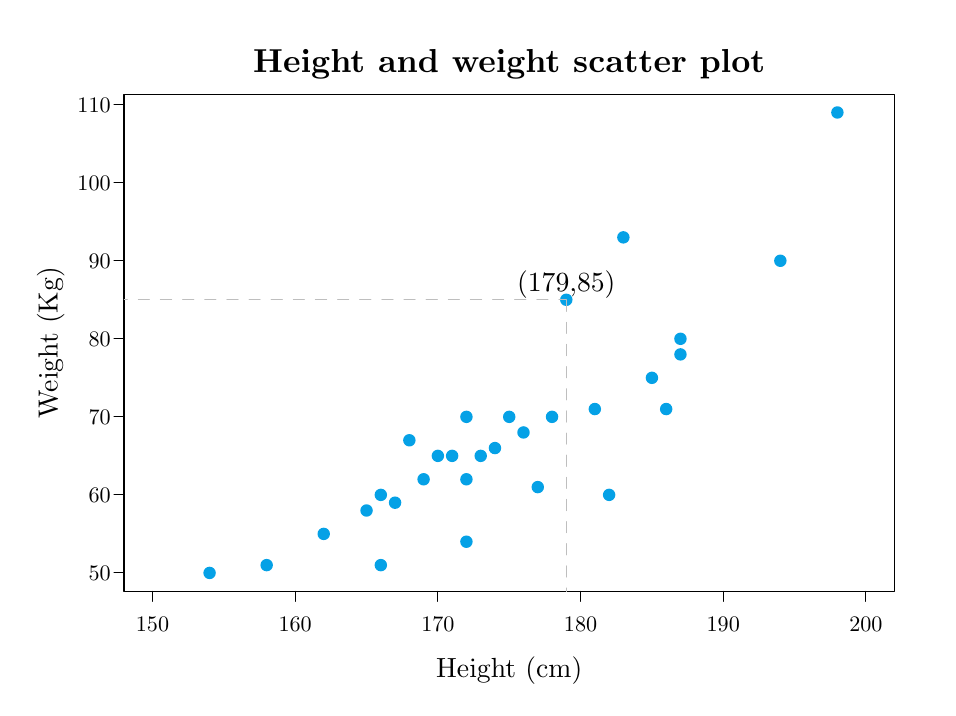
\begin{tikzpicture}[x=1pt,y=1pt]
\definecolor{fillColor}{RGB}{255,255,255}
\path[use as bounding box,fill=fillColor,fill opacity=0.00] (0,0) rectangle (325.21,238.49);
\begin{scope}
\path[clip] ( 34.80, 34.80) rectangle (313.21,214.49);
\definecolor{fillColor}{RGB}{5,161,230}

\path[fill=fillColor] (194.63,140.16) circle (  2.25);

\path[fill=fillColor] (163.70, 83.76) circle (  2.25);

\path[fill=fillColor] (204.94,100.68) circle (  2.25);

\path[fill=fillColor] (148.23, 83.76) circle (  2.25);

\path[fill=fillColor] ( 86.36, 44.28) circle (  2.25);

\path[fill=fillColor] (168.85, 86.58) circle (  2.25);

\path[fill=fillColor] (158.54, 75.30) circle (  2.25);

\path[fill=fillColor] (127.61, 69.66) circle (  2.25);

\path[fill=fillColor] (271.97,154.26) circle (  2.25);

\path[fill=fillColor] (225.57,111.96) circle (  2.25);

\path[fill=fillColor] (106.98, 55.56) circle (  2.25);

\path[fill=fillColor] (235.88,120.42) circle (  2.25);

\path[fill=fillColor] (292.59,207.84) circle (  2.25);

\path[fill=fillColor] (184.32, 72.48) circle (  2.25);

\path[fill=fillColor] (189.48, 97.86) circle (  2.25);

\path[fill=fillColor] (122.45, 64.02) circle (  2.25);

\path[fill=fillColor] ( 65.73, 41.46) circle (  2.25);

\path[fill=fillColor] (215.25,162.72) circle (  2.25);

\path[fill=fillColor] (127.61, 44.28) circle (  2.25);

\path[fill=fillColor] (153.38, 83.76) circle (  2.25);

\path[fill=fillColor] (174.01, 97.86) circle (  2.25);

\path[fill=fillColor] (210.10, 69.66) circle (  2.25);

\path[fill=fillColor] (132.76, 66.84) circle (  2.25);

\path[fill=fillColor] (143.07, 75.30) circle (  2.25);

\path[fill=fillColor] (158.54, 97.86) circle (  2.25);

\path[fill=fillColor] (230.72,100.68) circle (  2.25);

\path[fill=fillColor] (158.54, 52.74) circle (  2.25);

\path[fill=fillColor] (179.16, 92.22) circle (  2.25);

\path[fill=fillColor] (137.92, 89.40) circle (  2.25);

\path[fill=fillColor] (235.88,126.06) circle (  2.25);
\end{scope}
\begin{scope}
\path[clip] (  0.00,  0.00) rectangle (325.21,238.49);
\definecolor{drawColor}{RGB}{0,0,0}

\path[draw=drawColor,line width= 0.4pt,line join=round,line cap=round] ( 45.11, 34.80) -- (302.90, 34.80);

\path[draw=drawColor,line width= 0.4pt,line join=round,line cap=round] ( 45.11, 34.80) -- ( 45.11, 31.21);

\path[draw=drawColor,line width= 0.4pt,line join=round,line cap=round] ( 96.67, 34.80) -- ( 96.67, 31.21);

\path[draw=drawColor,line width= 0.4pt,line join=round,line cap=round] (148.23, 34.80) -- (148.23, 31.21);

\path[draw=drawColor,line width= 0.4pt,line join=round,line cap=round] (199.79, 34.80) -- (199.79, 31.21);

\path[draw=drawColor,line width= 0.4pt,line join=round,line cap=round] (251.34, 34.80) -- (251.34, 31.21);

\path[draw=drawColor,line width= 0.4pt,line join=round,line cap=round] (302.90, 34.80) -- (302.90, 31.21);

\node[text=drawColor,anchor=base,inner sep=0pt, outer sep=0pt, scale=  0.80] at ( 45.11, 20.40) {150};

\node[text=drawColor,anchor=base,inner sep=0pt, outer sep=0pt, scale=  0.80] at ( 96.67, 20.40) {160};

\node[text=drawColor,anchor=base,inner sep=0pt, outer sep=0pt, scale=  0.80] at (148.23, 20.40) {170};

\node[text=drawColor,anchor=base,inner sep=0pt, outer sep=0pt, scale=  0.80] at (199.79, 20.40) {180};

\node[text=drawColor,anchor=base,inner sep=0pt, outer sep=0pt, scale=  0.80] at (251.34, 20.40) {190};

\node[text=drawColor,anchor=base,inner sep=0pt, outer sep=0pt, scale=  0.80] at (302.90, 20.40) {200};

\path[draw=drawColor,line width= 0.4pt,line join=round,line cap=round] ( 34.80, 41.46) -- ( 34.80,210.66);

\path[draw=drawColor,line width= 0.4pt,line join=round,line cap=round] ( 34.80, 41.46) -- ( 31.21, 41.46);

\path[draw=drawColor,line width= 0.4pt,line join=round,line cap=round] ( 34.80, 69.66) -- ( 31.21, 69.66);

\path[draw=drawColor,line width= 0.4pt,line join=round,line cap=round] ( 34.80, 97.86) -- ( 31.21, 97.86);

\path[draw=drawColor,line width= 0.4pt,line join=round,line cap=round] ( 34.80,126.06) -- ( 31.21,126.06);

\path[draw=drawColor,line width= 0.4pt,line join=round,line cap=round] ( 34.80,154.26) -- ( 31.21,154.26);

\path[draw=drawColor,line width= 0.4pt,line join=round,line cap=round] ( 34.80,182.46) -- ( 31.21,182.46);

\path[draw=drawColor,line width= 0.4pt,line join=round,line cap=round] ( 34.80,210.66) -- ( 31.21,210.66);

\node[text=drawColor,anchor=base east,inner sep=0pt, outer sep=0pt, scale=  0.80] at ( 30.00, 38.70) {50};

\node[text=drawColor,anchor=base east,inner sep=0pt, outer sep=0pt, scale=  0.80] at ( 30.00, 66.90) {60};

\node[text=drawColor,anchor=base east,inner sep=0pt, outer sep=0pt, scale=  0.80] at ( 30.00, 95.10) {70};

\node[text=drawColor,anchor=base east,inner sep=0pt, outer sep=0pt, scale=  0.80] at ( 30.00,123.30) {80};

\node[text=drawColor,anchor=base east,inner sep=0pt, outer sep=0pt, scale=  0.80] at ( 30.00,151.50) {90};

\node[text=drawColor,anchor=base east,inner sep=0pt, outer sep=0pt, scale=  0.80] at ( 30.00,179.70) {100};

\node[text=drawColor,anchor=base east,inner sep=0pt, outer sep=0pt, scale=  0.80] at ( 30.00,207.90) {110};

\path[draw=drawColor,line width= 0.4pt,line join=round,line cap=round] ( 34.80, 34.80) --
	(313.21, 34.80) --
	(313.21,214.49) --
	( 34.80,214.49) --
	( 34.80, 34.80);
\end{scope}
\begin{scope}
\path[clip] (  0.00,  0.00) rectangle (325.21,238.49);
\definecolor{drawColor}{RGB}{0,0,0}

\node[text=drawColor,anchor=base,inner sep=0pt, outer sep=0pt, scale=  1.20] at (174.01,222.35) {\bfseries Height and weight scatter plot};

\node[text=drawColor,anchor=base,inner sep=0pt, outer sep=0pt, scale=  1.00] at (174.01,  3.60) {Height (cm)};

\node[text=drawColor,rotate= 90.00,anchor=base,inner sep=0pt, outer sep=0pt, scale=  1.00] at ( 10.80,124.65) {Weight (Kg)};
\end{scope}
\begin{scope}
\path[clip] ( 34.80, 34.80) rectangle (313.21,214.49);
\definecolor{drawColor}{RGB}{190,190,190}

\path[draw=drawColor,line width= 0.4pt,dash pattern=on 4pt off 4pt ,line join=round,line cap=round] (194.63,  0.00) -- (194.63,140.16);

\path[draw=drawColor,line width= 0.4pt,dash pattern=on 4pt off 4pt ,line join=round,line cap=round] (  0.00,140.16) -- (194.63,140.16);
\definecolor{drawColor}{RGB}{0,0,0}

\node[text=drawColor,anchor=base,inner sep=0pt, outer sep=0pt, scale=  1.00] at (194.63,143.30) {(179,85)};
\end{scope}
\end{tikzpicture}
